\documentclass[a4paper,12pt]{article}
\usepackage{amsmath, amssymb, graphicx}
\graphicspath{ {D:/Library/Meteorology/Note_tex} }

\DeclareMathAlphabet{\mathcal}{OMS}{cmsy}{m}{n}
\SetMathAlphabet{\mathcal}{bold}{OMS}{cmsy}{b}{n}
\newcommand{\bigO}{\mathcal{O}}


\begin{document}

\title{\vspace{-4.0cm}Thermal Wind}
\author{Ian Beckley
\\University of Wisconsin-Madison}

\date{13 Jan. 2021}

\maketitle

\subsection*{Thermal Wind}

The thermal wind describes how the geostrophic winds change with height. This vague definition allows two similar yet different mathematical representations, each useful in their own right. 

\subsubsection*{Differentiation of the Geostrophic Wind}

We begin with the zonal geostrophic wind, and subsequently substitute hydrostatic balance in order to define $u_g$ in terms of height.

\begin{align}
u_g = -\frac{1}{f\rho}\frac{\partial p}{\partial y}\\
u_g = -\frac{g}{f}\frac{\partial z}{\partial y}
\end{align}

Differentiating both sides with respect to pressure,

\begin{align}
\frac{\partial}{\partial p} u_g = \frac{\partial}{\partial p}(-\frac{g}{f}\frac{\partial z}{\partial y})\\
\frac{\partial u_g}{\partial p} = -\frac{g}{f}\frac{\partial}{\partial y}\frac{\partial z}{\partial p}
\end{align}

Recall that hydrostatic balance can also be written $\frac{\partial p}{\partial z} = -\frac{pg}{R_d T}$ using the IGL. Substituting into (4),

\begin{align}
\frac{du_g}{dp} = \frac{g}{f}\frac{\partial}{\partial y}\frac{R_d T}{pg}\\
\frac{\partial u_g}{\partial p} = \frac{R_d}{fp}\frac{\partial T}{\partial y}
\end{align}

Alternatively, we can express the LHS derivative in terms of $z$ with another substitution of hydrostatic balance.

\begin{align}
\frac{R_d T}{gp}\frac{\partial u_g}{\partial z} = \frac{R_d}{fp}\frac{\partial T}{\partial y}\\
\frac{\partial u_g}{\partial z} = \frac{g}{fT}\frac{\partial T}{\partial y}
\end{align}

Our final formulations include

\begin{align}
\boxed{\frac{\partial u_g}{\partial p} = \frac{R_d}{fp}\frac{\partial T}{\partial y}}\\
\boxed{\frac{\partial u_g}{\partial z} = \frac{g}{fT}\frac{\partial T}{\partial y}}\\
\boxed{\frac{\partial v_g}{\partial p} = -\frac{R_d}{fp}\frac{\partial T}{\partial x}}\\
\boxed{\frac{\partial v_g}{\partial z} = -\frac{g}{fT}\frac{\partial T}{\partial x}}
\end{align}

Note that via this definition, the thermal wind does not have typical wind units.

\subsubsection*{Vector Analysis}

The thermal wind can be alternatively be defined using vectors, where $\vec{V_T} = \vec{V_{upper}} - \vec{V_{lower}}$. While the formulations (9-12) explicitely defined the vertical speed shear of the environment, $\vec{V_T}$ describes the vector difference providing a useful window into vertical directional shear. Before delving into the implications of this view-point, let's expand upon the proposed vector difference.

Recalling that the geostrophic wind is $V_g = \frac{1}{f}\hat{k} \times \nabla_p \Phi$

\begin{align}
\vec{V_T} = \vec{V_2} - \vec{V_1} =  \frac{1}{f}\hat{k} \times \nabla_p (\Phi_2 - \Phi_1)
\end{align}

The hypsometric equation may be written $R_d T \ln{\frac{p_2}{p_1}} = (\Phi_2 - \Phi_1)$. Substituting into (13),

\begin{align}
\vec{V_T} = \frac{1}{f}\hat{k} \times \nabla_p \left[R_d T \ln{\frac{p_2}{p_1}}\right]\\
\vec{V_T} = \left[R_d \ln{\frac{p_2}{p_1}}\right]\frac{1}{f} \hat{k} \times \nabla_p T
\end{align}

While this is a result we could have assumed from (9-12), note that $\vec{V_T} \propto \nabla_p T \propto \nabla_p \Delta \Phi$, or that the thermal wind is proportional to the temperature/thickness gradient. Additionally, the right hand rule tells us that the thermal wind is always perpendicular to the temperature/thickness gradient with cold air/low thickness to the left. 

\subsubsection*{The Thermal Wind and Temperature/Thickness Advection}

Since the thermal wind is not a real wind, it cannot be responsible for physical advections such as temperature advection, nor should it due to orthogonality. Take, however, a veering profile such as that pictured below.
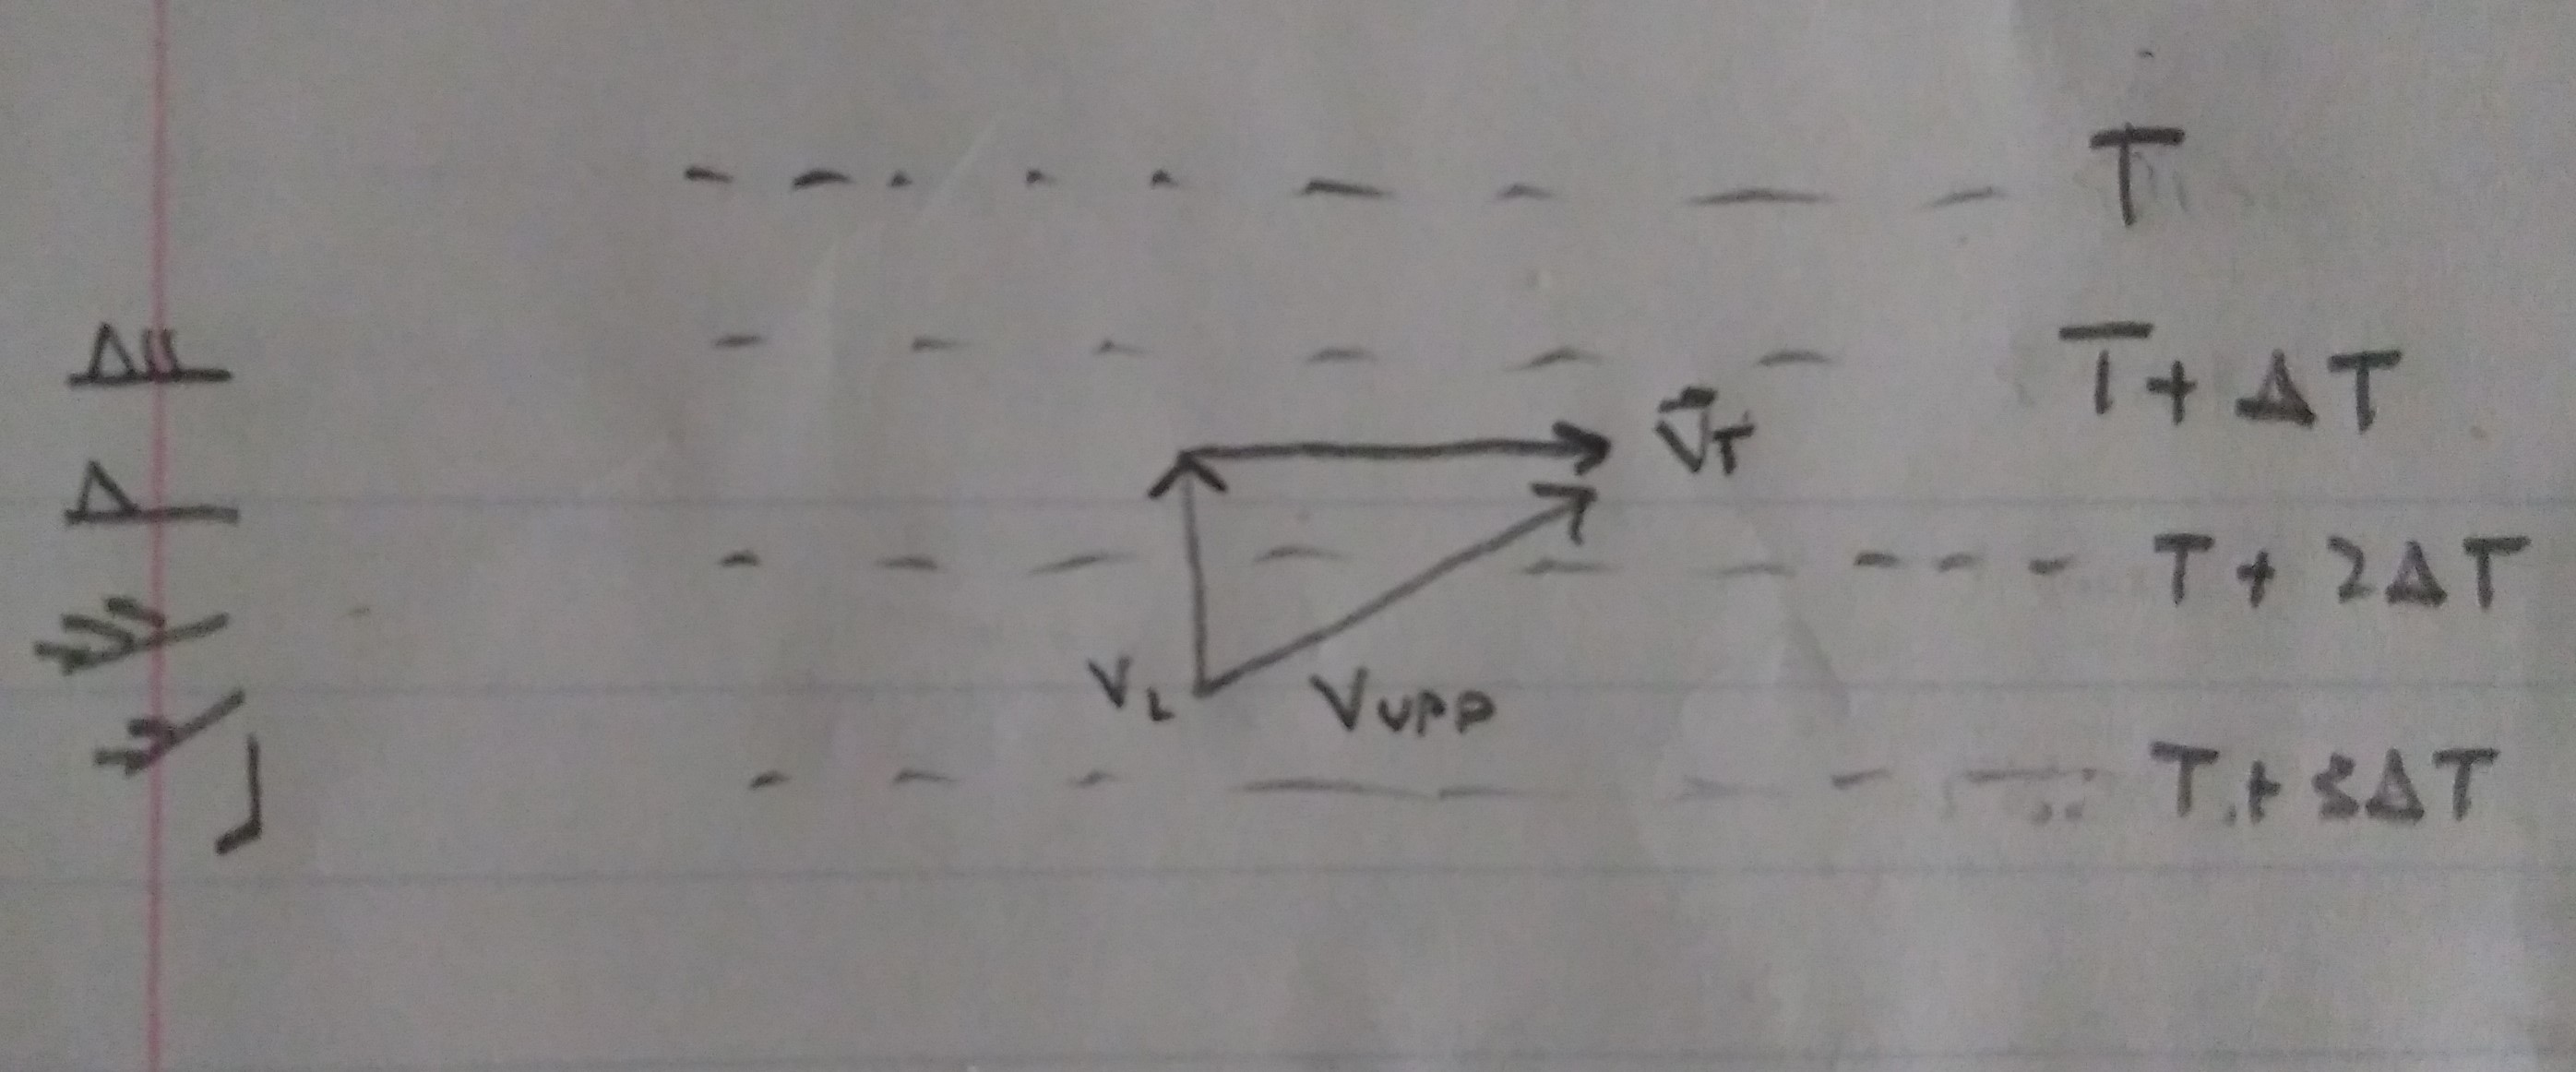
\includegraphics[width = \textwidth]{thermal_wind_1}

The thermal wind is cleary indicating the prescence of westerly shear in a north/south temperature gradient and blows with cold air to its left. The low-level geostrophic wind vector is scaled up for viewing, though clearly its southerly direction suggests warm air advection in the prescence of such a temperature gradient. The vertical wind profile is drawn to the left, confirming the prescence of low-level warm air advection and, by necesity, veering. This example illustrates the ubiquity of veering/backing with WAA/CAA in the mid-latitudes. If veering/backing does not exist, there can be no WAA/CAA (draw wind vectors and subtract them, none of them will cross isotherms). While this is a simplified example, be sure to take note of regions of vertical directional shear in atmospheric soundings when discussing the level at which temperature advections are actually occuring. 


\end{document}